
\documentclass[UTF8, onecolumn, a4paper, 12pt]{article}
\usepackage{ctex}
\usepackage{geometry}
\usepackage{amsmath}
\usepackage{multirow, multicol}
\usepackage{subfig}
\usepackage{float}
\usepackage{graphicx}
\usepackage{lettrine}
\usepackage{authblk}
\usepackage{xcolor}%用于设置颜色
\usepackage{fontspec}
\usepackage{setspace}
\usepackage{verbatim}
\geometry{left=1.0cm,right=1.0cm,top=1.0cm,bottom=1.0cm}

\title{中级宏观经济学笔记}%———总标题
\author{Liu Hongzun}
\affil{Department of Computer Science, Tsinghua University}
\date{2020.02 - 2020.06}
\renewcommand{\baselinestretch}{0.9}
\begin{document}
%\maketitle %输入此句才会显示标题
\setlength\columnseprule{0.2pt}
\section{Chapter 1: Introduction and Basic Knowledge}
\subsection{研究问题}
1.长期经济增长的影响因素
2.名义价格和通胀的影响因素
3.短期经济波动的影响因素(经济周期理论)
4.国际贸易的影响因素(开放市场理论)
\subsection{模型}
抽象、简单、区分内生变量和外生变量、可验证.
\subsection{Short run}
固定的资本、价格、技术水平
\subsection{Long run}
价格调整、资本积累、技术进步、市场出清

$\bullet$外生变量和内生变量依赖于模型
$\bullet$宏观经济没有办法做实验
$\bullet$凯恩斯主义是短期的,不是长期的
\subsection{数据(measurement, statistic, data)}
\subsubsection{Stock \& Flow}
存量 \& 流量\\
$$K_{t+1} = (1 - \delta)K_t + l_t$$
k:存量, l:流量, $\delta$折旧 率(贬值率)
\subsubsection{GDP: Gross Domestic Product}
国内生产总值:包括外国人的投资。\\
一年或一个季度中{\bfseries 一国国内}新生产的{\bfseries 最终商品}和{\bfseries 最终服务}的{\bfseries 市场价值}。
不计算中间物品!!!是流量!!!
$$GDP = P_t^AQ_t^A + P_t^BQ_t^B+\cdots$$
$\bullet$合理估价!!!当年自建物品也要算在其中。\\
$\bullet$政府服务,公共教育服务都没有市场价格,但是要算在其中。\\
$\bullet$生产出来但是没有卖出,仍应算在GDP中\\
$\bullet$已经被使用过的物品(不是当年生产的)不计入GDP\\
$\bullet$房子计入GDP,但是汽车、家电等不计入其中。因为汽车、家电等对GDP的贡献十分少。但租车依然计入GDP(租车公司提供了服务)。\\
$\bullet$ GDP不计入地下经济(黑色资金)\\
$\bullet$非市场活动不计入:打扫自家卫生(不计入),雇佣小时工(提供服务,计入)\\
$\bullet$交易二手物品不计入GDP,如果存在交易中介获取佣金就计入这部分\\
$\bullet$居住在房内:房子对自己产生了服务,计入GDP;买了房子但是不住在其中,没有对自己产生服务,实际上不应计入,但是无法调查,所以国家将其计入GDP!!!\\
$\bullet$ financing.金融活动不影响GDP,即不管是贷款还是融资买房,GDP都计入房子的价格\\
$\bullet$购买商品所交的税款,要么归入消费,要么归入政府支出(由税收提供),不能重复计算收税。\\
$\bullet$人均$GDP$: \textit{GDP Per Capita}\\
真实$GDP$(以$b$为基年价格)\textit{\textbf{Fixed Price, Changed Goods}}:
$$RGDP_t = P_b^AQ_t^A + P_b^BQ_t^B + \cdots$$
名义$GDP$(以当年$t$为价格):
$$NGDP_t = P_t^AQ_t^A + P_t^BQ_t^B + \cdots$$
年均增长率:
\begin{equation}
\begin{aligned}
Aver\quad Growth &= \sqrt[t-b]{\frac{RGDP_t}{GDP_b}} - 1 \\&= \sqrt[t-b]{\frac{P_b^AQ_t^A + P_b^BQ_t^B + \cdots}{P_b^AQ_b^A + P_b^BQ_b^B + \cdots}} - 1
\end{aligned}
\end{equation}
$\bullet$ GDP的基年会定时进行修正,基年价格也会随之改变。\\
$\bullet$国家之间的比较:
$$NGDP_{Japan}^{dollars} = NGDP_{Japan}^{yen} / E$$  
where \textit{\textbf{E}} is the \textit{\textbf{Average Nominal Exchange Rate}} of how many \textit{yen} you can buy with a \textit{dollar}.
\subsubsection{GNP: Gross National Product}
国民生产总值:国内国民的收入,外国人的生产不算\\
$\bullet$即中国人在国外生产的价值计入中国GNP,外国人在中国生产的价值不计入中国GNP\\
$\bullet$如果国外厂商所占国内资产所占比重大,则GDP>GNP(中国略大).
\subsubsection{GNI: Gross National Income}
国民总收入:不包括外国人的收入。
\subsubsection{PPP: Purchasing Power Parity exchange rates}
购买力平价\\
类似CPI,采用篮子来衡量,由国内和国外两部分构成。\\
$PPP$计算$GDP$,一般会使得发展中国家的GDP被显著提升。因为发展中国家的人力资源比较廉价。
\subsection{Inflation}
\subsubsection{GDP deflator}
$$P_t = \frac{NGDP_t}{RGDP_t}$$
\subsubsection{CPI: Consumer Price Index}
消费者物价指数\\
\textit{A bucket of goods(\textbf{Fixed Goods, Changed Price}):}
$$CPI = \frac{P_t^AQ_b^A + P_t^BQ_b^B + \cdots}{P_b^AQ_b^A + P_b^BQ_b^B + \cdots}$$
$\bullet$只包括消费品,不包括所有的物品(如投资品,建筑等).\\
$\bullet$包括进口商品。而GDP不包括。\\
$\bullet$篮子是固定的。\\
$\bullet$不能cover所有的商品,不能跟踪商品结构变化。\\
$\bullet$存在Subtitution Bias:篮子中每个商品的个数是固定的,不能实时调节比例。当商品存在替代品的时候,通胀对国民经济的影响其实没有CPI体现的那么严重。这会使得:计算所得CPI高于真实的CPI。\\
$\bullet$ New Goods:无法体现新产品的影响。\\
$\bullet$无法体现质量(Quality)上的变动:比如电脑的更新换代,但是价格基本不变。无法反应生活质量的变化。这会使得:计算所得CPI高于真实的CPI。\\
$\bullet$ GDP deflator 所反映的通胀程度波动幅度低于CPI。
\paragraph{Deficit: 赤字}
\section{Chpater 2: Production, Income and Expenditures}
\textit{Y = \textbf{GDP} = \\ value added of all \textbf{goods and service} = total \textbf{income} = total \textbf{expenditure on final goods}}
\subsection{Production}
三个产业提供价值的加总:\\
\textbf{GDP} = Value Added in all sectors = Value Added in \textbf{Agriculture}(Primary) + Value Added in \textbf{Manufacturing \& construction}(Secondary) + Value Added in \textbf{Services}(Tertiary)
$$Y = Y_{ag} + Y_{mfg} + Y_{ser}$$
\begin{figure}[htb]
	\centering
	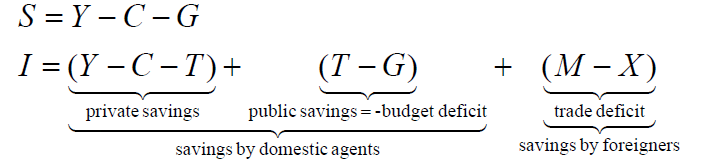
\includegraphics[width=0.9\linewidth]{GDP}
\end{figure}
\subsection{Income}
\textbf{GDP} = income to everyone in the economy = \textbf{Capital Income + Labor Income}\\
$\bullet$ Capital Inequality \& Income Inequality
\subsection{Expenditure}最终花费(\textbf{final})
$$Y = C + I+G+(X-M) = C + I + G + NX$$
$$NX = Y - C - I - G$$
$$S = Y - C - G$$
$$I = (Y - C - T)_{PrivateSaving} + (T -G)_{PublicSaving} + (M - X)_{TradeDeficit(ForeignSaving)}$$
$$I - S = M - X$$
C:消费, I: 投资(修建铁路、厂房、机器等。是经济意义上的投资) G: 政府购买
X: 出口, M:进口, NX:净出口, T: Tax, (M-X): 外国人投资在该国的货币\\
$\bullet$ $I-S$反映了一个国家的开放程度,如果完全开放的话,$S = I$\\
$\bullet$ $M < X$,净出口为正,相当于自己在国外的投资。$M > X$,净出口为负,相当于外国人在国内的投资。\\
$\bullet$大部分是消费。\\
$\bullet$现代经济中储蓄等于投资,相当于钱不会存在家里,都在银行。\\
$\bullet$金融行业投资是有债权人和债务人的,和经济的投资是不同的。\\
\textbf{Contraction in Output}: 产出收缩.
\section{宏观经济模型}
\subsection{Preparing Konwledge}
\paragraph{生产函数(Neoclassical Production Function)}
参数:

产出: Y, 资本存量: K, 劳动力: L, 知识或劳动效率(ideas, patents, and R\&D): A; 

人均产出$y$, 人均资本$k$, 人均消费$c$, 人均投资$i$, 储蓄率$s$, 折旧率$\delta$.
$$Y = A\cdot F(K, L)$$
曲线上凸, 过零斜率无穷.
\paragraph{投入要素}
人口和技术按指数增长. 
人口增长率$$\frac{\triangle L_t}{L_t} = n$$ 技术进步率$$\frac{\triangle E_t}{E_t} = g$$
\paragraph{国民收入核算恒等式}
$$y = c + i$$
\paragraph{消费函数}
$$c = (1 - s)y$$
设产品价格$P$, 单位劳动报酬$W$, 单位资本开销$R$. 企业选择最优化:
$$\max_{K,L} PAF(K,L) - WL - RK$$
一阶条件:
$$P\frac{\partial AF(K,L)}{\partial K} - R = 0$$
$$P\frac{\partial AF(K,L)}{\partial L} - W = 0$$
进而得到
\paragraph{MPK}资本的边际产量. ($MPK$递减)
$$MPK = \frac{\partial AF(K,L)}{\partial K} = r = \frac{R}{P}$$
\paragraph{MPL}劳动的边际产量. 
$$MPL = \frac{\partial AF(K,L)}{\partial L} = w = \frac{W}{P}$$
其中$w$为劳动租赁价格, $r$为资本租赁价格. 
\subsection{Cobb-Douglas Production Function}
$$Y = AF(K, L) = AK^{\alpha}L^{1-\alpha}$$
满足“规模不变报酬”性质.  上式取对数后求微分:
$$\frac{\triangle Y}{Y} = \frac{\triangle A}{A} +\alpha \frac{\triangle K}{K} + (1 - \alpha)\frac{\triangle L}{L}$$
$$y = \frac{Y}{L} = Ak^{\alpha}$$
\paragraph{TFP}total factor productivity, 全要素生产率:
$$TFP = \frac{\triangle A}{A}$$
且此时:
$$MPK = \frac{\partial AF(K,L)}{\partial K} = \alpha\frac{Y}{K} = r$$
$$MPL = \frac{\partial AF(K,L)}{\partial L} = (1-\alpha)\frac{Y}{L} = w$$
\textbf{预测:} 工资增长率 = 劳动的边际产量.
\paragraph{Labor Share of Income}
劳动收入份额. 
$$laborshare = \frac{WL}{PY} = \frac{W}{P}\frac{L}{Y} = MPL\frac{L}{Y}$$
代入Cobb-Douglas Production Function:
$$laborshare = MPL\frac{L}{Y} = (1-\alpha)\frac{Y}{L}\frac{L}{Y} = 1 - \alpha$$
\textbf{Labor Share Constant!}
\paragraph{Capital Share of Income}
资本收入份额. 
$$capitalshare = \frac{RK}{PY} = \frac{R}{P}\frac{K}{Y} = MPK\frac{K}{Y}$$
代入Cobb-Douglas Production Function:
$$capitalshare = MPK\frac{K}{Y} = \alpha\frac{Y}{K}\frac{K}{Y} = \alpha$$
\textbf{Capital Share Constant!}

得到重要结论:
$$1 = laborshare + capitalshare$$
$$Y = (1-\alpha)\frac{Y}{L}\cdot L + \alpha\frac{Y}{K}\cdot K = MPK\cdot K + MPL\cdot L = \frac{WL}{P} + \frac{RK}{P}$$
\textbf{没有经济利润!}
\subsection{货币恒等式}
$$MV = PY$$
$V$: 货币流通速度; $M$: 货币总量

$\mu$: 货币供给净增长率; $\pi$: 净通胀率(增长); $g$: GDP增长率.
\textbf{货币中性论:} 货币供给只影响价格水平,不影响真实变量.
$$\frac{\triangle M}{M} + \frac{\triangle V}{V} = \frac{\triangle P}{P} + \frac{\triangle Y}{Y}$$
$$\mu = \pi + g$$
\textbf{假设:} $g$和$\mu$独立, $V$固定.

\paragraph{Fisher Equation}
$r$: 实际利率, $i$: 名义利率.
$$\pi_{t} = P_{t}/P_{t-1}  - 1$$
$$(1 + r_t)(1+\pi_{t+1}) = 1+i_t$$
近似得到:
$$i_t = r_t + \pi_{t+1}$$
长期均衡:
$$i = r + E\pi$$
$$\frac{M}{P} = \frac{Y}{V(i)} = L(i, Y) = L(r + E\pi, Y)$$
名义利率$i$越高, 持有货币的成本越高,货币流通速度$V$越高,$M/P$下降.

\paragraph{supply and demand}
存款: $D$, 现金:$C$, 银行准备金:$R$
$$M = C+ D$$
实际货币(controlled by the central bank)$B = C+ R$

准备金率(ratio of reserves to deposits):$rr = \frac{R}{D}$

货币存款比率(Currency-deposit ratio, depends on households’ preferences):$cr= \frac{C}{D}$

货币乘数:$$m = \frac{C+D}{B} = \frac{C+D}{C+R} = \frac{cr+1}{cr+rr}$$
$rr<1$, 所以$m>1$.
$$M = C+D =  \frac{C+D}{B}B = m B$$
\paragraph{变动}
Loss of confidence in banks: $cr$上升.
Banks became more cautious: $rr$上升.

\subsection{Simple Model}
封闭经济体:
$$Y = C + G + I$$
消费取决于可支配收入:
$$C = a + b(Y-T)$$
投资受利率影响:
$$I = c - dr$$
政府变量外生给定:
$$G = G, T = T$$
产出不变:
$$Y = Y$$
得到方程:
$$dr = a+b(Y- T) - Y + c +G$$
\subsection{Solow Model}
Solow 模型通过假定一系列外生参数,尤其是固定不变的储蓄率$s\in (0, 1)$,利用生产函数的函数性质得到一个违背我们直觉但又在常理之中的结论:在长期,有效人均资本量$k$、产出$y$及消费量$c$都将维持在某一个不变的值,即稳定状态。并且总产出的增长只来源于人口增长率$n$和技术进步率$g$.
\paragraph{假设} 生产函数有规模不变报酬. 即$\forall z, zY = F(zK, zL)$. 进而有人均产出
$$y = Y/L = AF(K/L, 1) := Af(k)$$

\paragraph{资本动态方程}
投资 = 储蓄:
$$i = sy = sf(k)$$
资本存量按折旧率损失:
$$\triangle k = i - \delta k = sf(k) - \delta k = savings - depreciation$$
\paragraph{稳态}
令$\triangle k = 0$, 得到稳态$k^*$
$$sf(k^*) = \delta k^*$$
给定$s, f(\cdot), \delta$可以计算稳态.
\paragraph{引入人口增长率$n$}
$$\triangle k = \frac{\triangle K}{L} - n$$
$$\triangle k = sf(k) - (\delta + n)k$$
\textbf{引入技术/效率$E$, 增长率$g$:} $$Y = F(K, EL)$$
得到:
$$sf(k^*) = (\delta + n + g)k^*$$
\textbf{修正原模型:}
$$y = \frac{Y}{EL}$$
$$k = \frac{K}{EL}$$
即$K/L = kE$.

对于Cobb-Douglas Production Function稳态:
$$sf(k^*) = sAk^{\alpha} = (\delta + n + g)k^*$$
得到
$$k^* = \sqrt[1-\alpha]{\frac{sA}{\delta + n + g}}$$
\paragraph{黄金率}
社会福利用消费衡量,使得消费最大化的$k^*$:
$$\max_{k^*}c^* = (1-s)y^* = f(k^*) - sf(k^*) = f(k^*) - (\delta + n + g)k^*$$
一阶条件:
$$\frac{\partial c^*}{\partial k^*} = f'(k^*) - (\delta + n + g)$$
即黄金率值$k^G$:
$$f'(k^G) = (\delta + n + g)$$
对于Cobb-Douglas Production Function:
$$k^* = \sqrt[1-\alpha]{\frac{sA}{\delta + n + g}}$$
进而有:
$$s^{G} = (\delta + n + g)(k^G)^{1-\alpha} / A$$
$k^G$和$s^G$同步变动.
\subsubsection*{储蓄率$s$发生变动}
\begin{enumerate}
	\item 对$k^*$的影响
	
	我们对均衡等式$s f\left(k^{*}(s, n, g, \delta)\right)=(n+g+\delta) k^{*}(s, n, g, \delta)$两端同时关于$s$求一阶导,
	\begin{align}
	s f^{\prime}\left(k^{*}\right) \frac{\partial k^{*}}{\partial s}+f\left(k^{*}\right) = 
	(n+g+\delta) \frac{\partial k^{*}}{\partial s}
	\end{align}
	整理得到
	\begin{align}\label{solowpartialks}
	\frac{\partial k^{*}}{\partial s} = \frac{f\left(k^{*}\right)}{(n+g+\delta)-s f^{\prime}\left(k^{*}\right)}
	\end{align}
	\item 对$y^*$的影响
	
	由$y=f(k)$,有
	\begin{align}
	\frac{\partial y^{*}}{\partial s} = 
	f^{\prime}\left(k^{*}\right) \frac{\partial k^{*}(s, n, g, \delta)}{\partial s}
	\end{align}
	将式(\ref{solowpartialks})结果带入,整理得到
	\begin{align}
	\frac{\partial y^{*}}{\partial s} = 
	\frac{f^{\prime}\left(k^{*}\right) f\left(k^{*}\right)}{(n+g+\delta)-s f^{\prime}\left(k^{*}\right)}
	\end{align}
	$s$上升, $k$或$y$逐渐上升至稳定.
	
	\item 对$c^*$的影响
	
	由定义,$c=(1-s)y$,且稳态下有$sf(k^*) = (n+g+\delta)k^*$,故得到
	\begin{align}
	c^{*} = f\left(k^{*}\right)-(n+g+\delta) k^{*}
	\end{align}
	对其两端求导,整理得到
	\begin{align}
	\frac{\partial c^{*}}{\partial s} = 
	\left[f^{\prime}\left(k^{*}\right)-(n+g+\delta)\right] 
	\frac{\partial k^{*}(s, n, g, \delta)}{\partial s}
	\end{align}
	将式(\ref{solowpartialks})结果带入,得到
	\begin{align}
	\frac{\partial c^{*}}{\partial s} = 
	\left[f^{\prime}\left(k^{*}\right)-(n+g+\delta)\right] 
	\frac{f\left(k^{*}\right)}{(n+g+\delta)-s f^{\prime}\left(k^{*}\right)}
	\end{align}
	$s$上升,$c$先突然下降,后逐渐上升.
\end{enumerate}
\subsubsection{趋同}
开始时落后的国家可以“赶上”领先的国家.

根据Solow模型,两个经济体是否趋同取决于它们的初始状态. 假设一开始两个经济体因为历史偶然性导致资本存量$K$不同,但是他们有着储蓄率$s$,人口增长率$n$和技术效率$g$决定的\textbf{相同的稳态},我们预期这两个经济体应该趋同; 在到达稳态的过程中,有更少资本存量$K$的经济体增长将更快(如德国和日本战后的快速增长); 如果稳态不同,那么他们将不趋同.

\subsubsection{条件趋同(Conditional Convergence)}
具有不同初始收入水平但是有相似的经济政策和制度的经济随着时间的推移在收入上变得更加相似. 

储蓄率$s$,人口增长率$n$和技术效率$g$等条件将不同国家引导向不同的稳态,但是稳态又都由储蓄、人口增长和人力资本等变量决定,这种现象叫“条件趋同”.


绝对趋同是指人均收入(人均资本)较低的国家或地区其人均指标的增速总是快于较高的国家或地区,比如中国与美国。 条件趋同讲的是上述趋同是有条件的,即要求稳态时人均指标相同,如果人均指标较高的国家或地区具有较高的稳态指标,那么有可能人均指标较低的国家其增速慢于较高的国家。 

\textbf{产出冲击:} $y$下降,$c, i$同步下降.
\begin{center}
	\begin{figure}[htb] %强制单栏排版
		\centering %居中
		\begin{minipage}[b]{\linewidth}
			\subfloat[]{
				\begin{minipage}[b]{0.46\linewidth} 
					\centering
					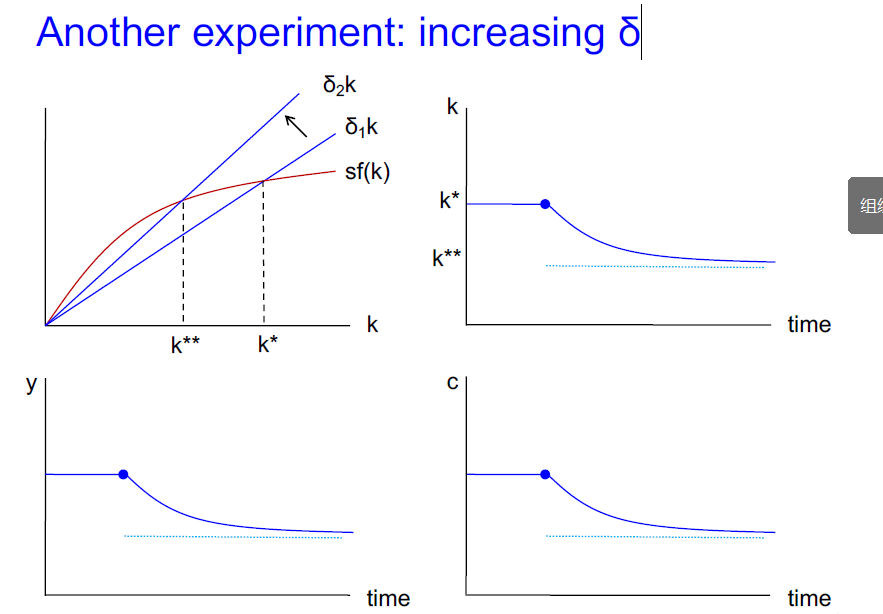
\includegraphics[width=\linewidth]{delta}\vspace{8pt}
					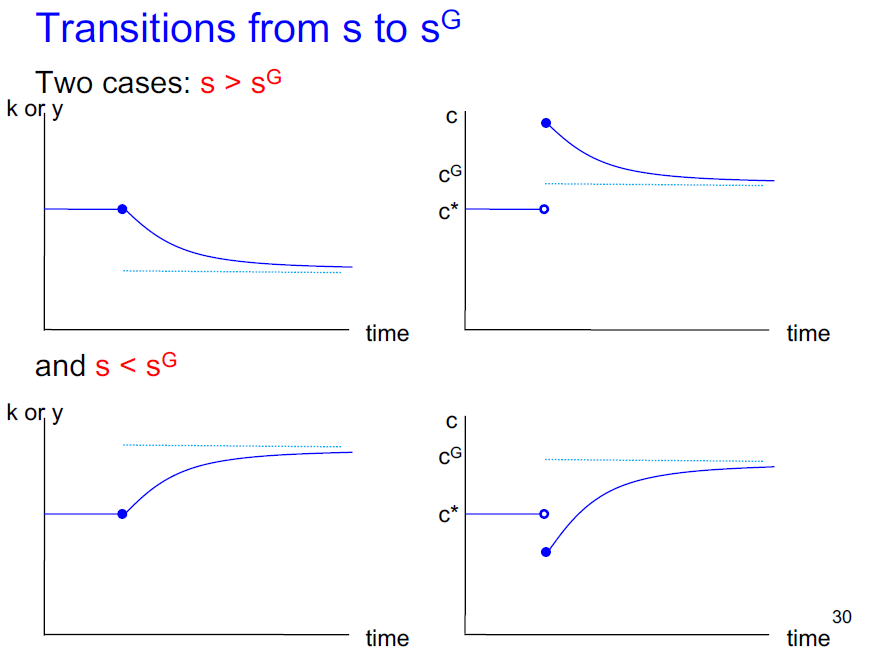
\includegraphics[width=\linewidth]{saving}
				\end{minipage}
			}\
			\hfill
			\subfloat[]{
				\begin{minipage}[b]{0.46\linewidth}
					\centering
					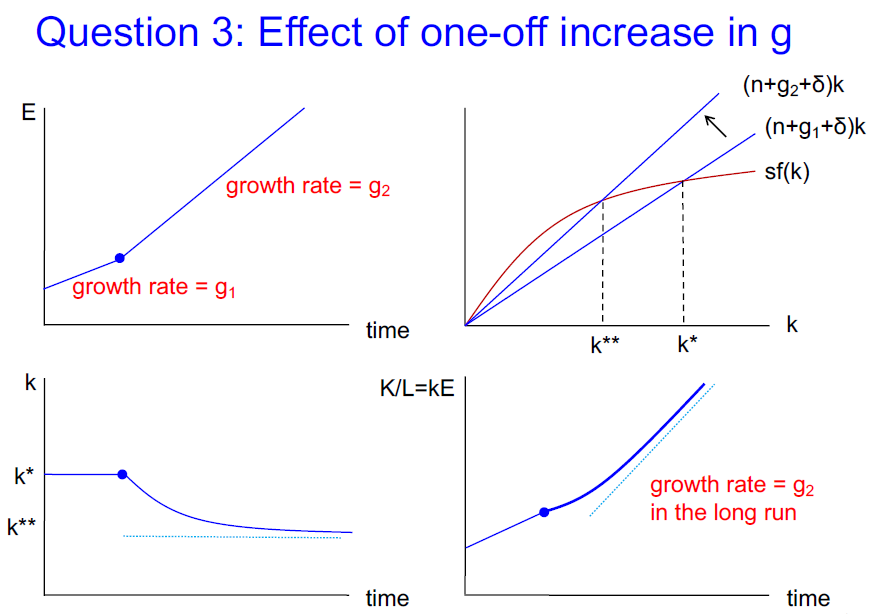
\includegraphics[width=\linewidth]{g}\vspace{8pt}
				\end{minipage}
			}
		\end{minipage}
	\end{figure}
\end{center}
\subsection{AK-Model}
$$Y = AK$$
$$\triangle k = sAk - (\delta+n+g) k$$
\subsection{Two-Sector Model}
投入到R\&D的劳动比例$u$, 投入到生产的劳动比例$1-u$.
$$Y = K^{\alpha}[(1-u)EL]^{1-\alpha}$$
$$y = \frac{Y}{EL} = k^{\alpha}(1-u)^{1-\alpha}$$
技术积累:
$$\triangle E = g(u)E$$
资本积累:
$$\triangle K = sY - \delta K$$
$$\triangle k = \triangle\frac{K}{EL} = \frac{\triangle K}{EL} - K\frac{\triangle E}{E}= sy - \delta k - g(u)k$$
其中$k = K/EL$,求导得到:
$$\frac{\triangle k}{k} = sk^{\alpha-1}(1-u)^{1-\alpha}-\delta -g(u)$$

\subsection{IS-LM Model}
\paragraph{两个市场}
\textbf{直观理解:}产品市场上,利率越低,投资越多,拉动GDP越多; 货币市场上,GDP越高,货币需求越大,而货币供给不足,只能提高利率减小需求.

\textbf{(LM)货币市场:}
$$MV(i) = MV(r+E\pi)=PY$$
$$\frac{M}{P} = L(r+E\pi, Y) := Y - k(r+E\pi)$$
\textbf{得到LM Curve:}
$$r = \frac{1}{k}Y - E\pi - \frac{1}{k}\frac{M}{P}$$

\textbf{(IS)商品市场:}
$$S = I$$
$$(Y-C-G) + (T-G) = I$$
$$Y = C+I+G$$
$$C = a+b(Y-T)$$
$$I = c-dr$$
得到:
$$Y = a+b(Y-T)+c-dr + G$$
$$\triangle Y = b\triangle Y + \triangle G$$
所以有政府购买乘数效应(The government-purchases multiplier):
$$\triangle Y = \triangle G\frac{1}{1-b}$$
税收乘数(tax multiplier):
$$\triangle Y = b(\triangle Y - \triangle T)$$
$$\triangle Y= -\triangle T\frac{b}{1-b}$$
\textbf{得到IS Curve:}
$$r = -\frac{1-b}{d}Y + \frac{1}{d}(a+c+G-bT)$$
Higher real interest rates, lower investment, lower output.
\paragraph{IS-LM}
$$r = -\frac{1-b}{d}Y + \frac{1}{d}(a+c+G-bT) \quad(IS)$$
$$r = \frac{1}{k}Y - E\pi - \frac{1}{k}\frac{M}{P} \quad(LM)$$
\textbf{稳态:}
$$Y = \frac{1}{1-b+d/k}(G - bT +\frac{d}{k}\frac{M}{P} +a +c + dE\pi)$$
\textbf{Fiscal Policy:}
$$\triangle Y = \frac{1}{1-b+d/k}\triangle G$$
\textbf{Monetary Policy:}
$$\triangle Y = \frac{1}{1-b+d/k}\frac{\triangle M}{P}$$
\textbf{相关乘数:}
$$\frac{\triangle Y}{\triangle G} = \frac{1}{1-b+d/k}$$
$$\frac{\triangle C}{\triangle G} = \frac{b}{1-b+d/k}$$
\subsubsection{动态变动}
在动态变动中,联邦银行应保持利率$r$不变, 需要调节货币供给$M$.
\paragraph{Animal Spirits} 人们的行为并不理性,使得$a, c$下降,$IS$曲线下降.
\paragraph{Liquidity Trap} 流动性陷阱(凯恩斯提出)。当一定时期的利率水平降到不能再低时,人们便会预期利率上升,货币需求弹性变得无限大,即无论增加多少货币,人们都会选择储蓄,而利率几乎不变(k趋于无穷). 此时货币政策失效.
\paragraph{Relative efficiency of fiscal versus monetary}
$$\frac{\triangle Y/\triangle G}{\triangle Y/\triangle M} = \frac{\frac{1}{1-b+d/k}}{\frac{d/k}{1-b+d/k}\frac{1}{P}} = \frac{Pk}{d}$$
So \textbf{fiscal policy} more powerful if $k > d$ and \textbf{monetary policy} more powerful otherwise
\begin{figure}[htb]
	\centering
	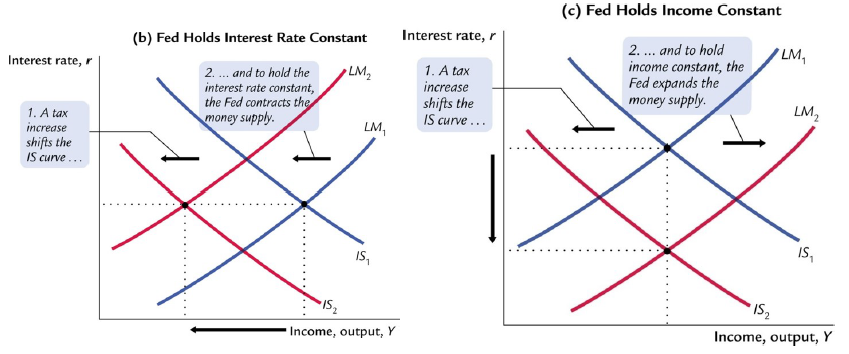
\includegraphics[width=0.6\linewidth]{fed}
	\caption{货币政策和财政政策的互动}
\end{figure}
\begin{center}
	\begin{figure}[htb] %强制单栏排版
		\centering %居中
		\begin{minipage}[b]{\linewidth}
			\subfloat[]{
				\begin{minipage}[b]{0.46\linewidth} 
					\centering
					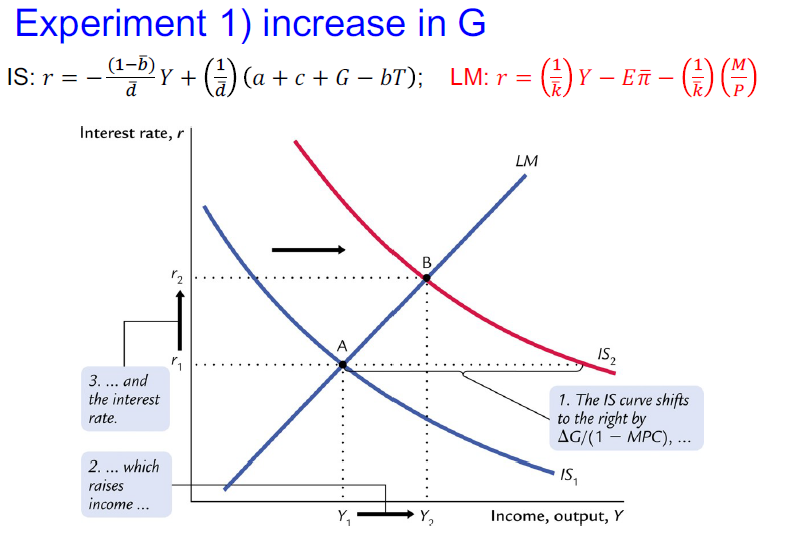
\includegraphics[width=\linewidth]{inG}\vspace{8pt}
					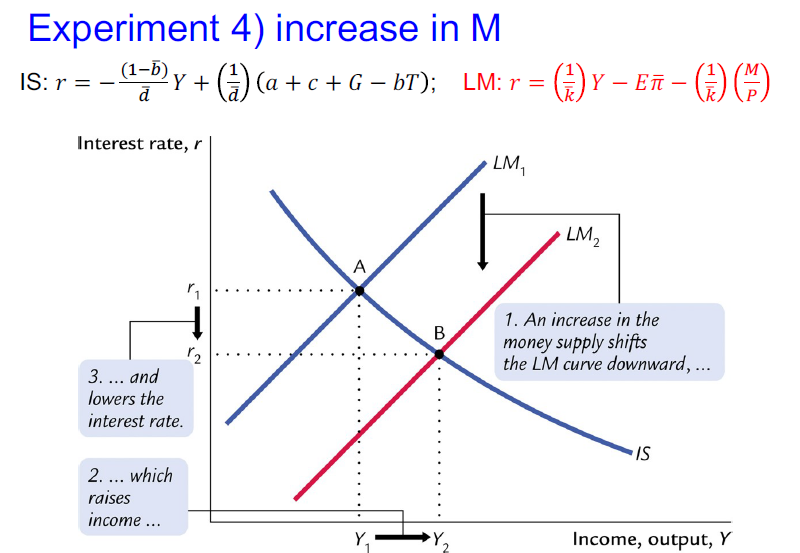
\includegraphics[width=\linewidth]{inM}
				\end{minipage}
			}\
			\hfill
			\subfloat[]{
				\begin{minipage}[b]{0.46\linewidth}
					\centering
					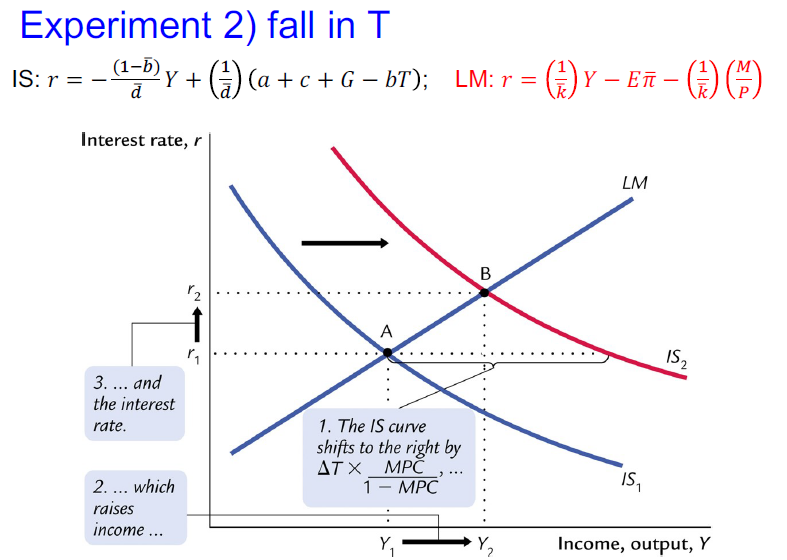
\includegraphics[width=\linewidth]{faT}\vspace{8pt}
					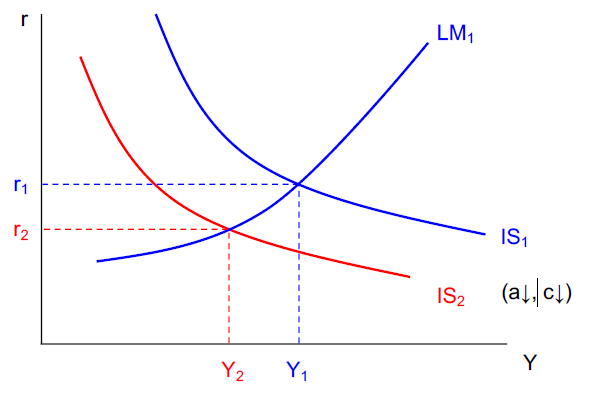
\includegraphics[width=\linewidth]{animal}
					\caption{Animal Spirit}
				\end{minipage}
			}
		\end{minipage}
	\end{figure}
\end{center}
\begin{center}
	\begin{figure}[htb] %强制单栏排版
		\centering %居中
		\begin{minipage}[b]{\linewidth}
			\subfloat[]{
				\begin{minipage}[b]{0.4\linewidth} 
					\centering
					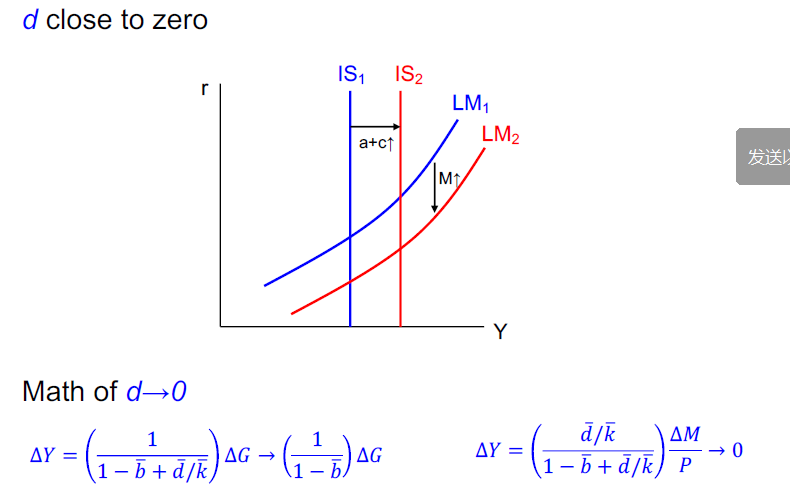
\includegraphics[width=\linewidth]{d_low}
					\caption{d非常小时, IS曲线垂直}
					\vspace{8pt}
					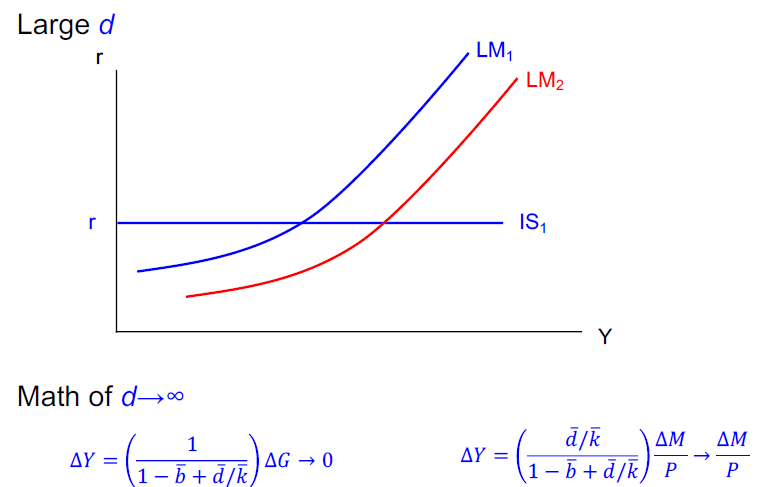
\includegraphics[width=\linewidth]{d_high}
					\caption{d非常大时, IS曲线水平,Fiscal Policy失效}
				\end{minipage}
			}\
			\hfill
			\subfloat[]{
				\begin{minipage}[b]{0.5\linewidth}
					\centering
					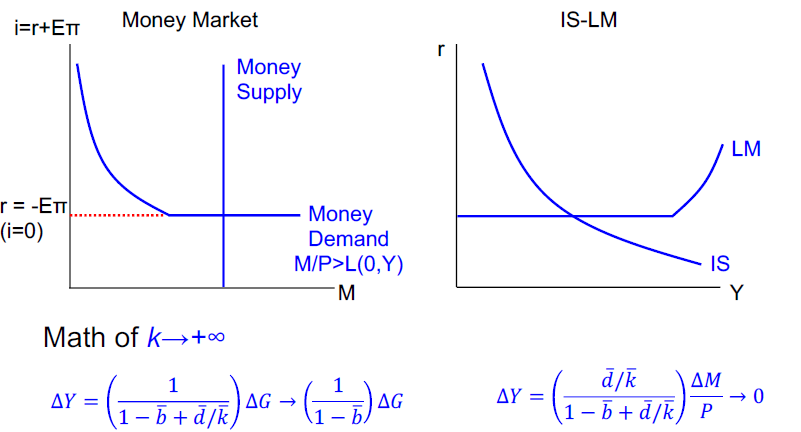
\includegraphics[width=\linewidth]{liquidity_trap}
					\caption{Liquidity Trap}
					\vspace{8pt}
					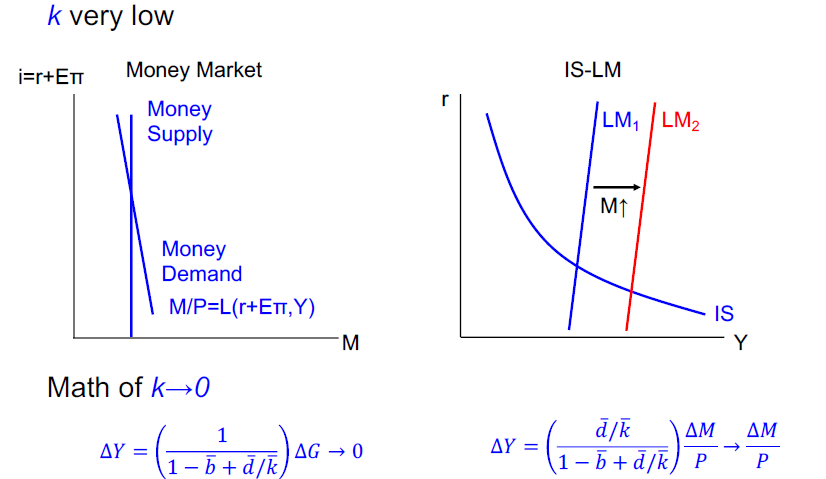
\includegraphics[width=\linewidth]{k_low}
					\caption{k非常小时}
				\end{minipage}
			}
		\end{minipage}
	\end{figure}
\end{center}
\subsection{AS-AD Model: 短期}
Get rid of fixed P assumption. $P$上升时, LM曲线上升,产出$Y$下降. 所以$P, Y$负相关.

\textbf{Aggregate Demand Curve: P-Y}

\textbf{Aggregate Supply Curve: P-Y}

\textbf{黏性价格模型:} 需要考虑具有弹性价格的企业比例1-s, 和具有黏性价格的企业比例s.
$$P = sEP + (1-s)[P + a(Y-\overline{Y})]$$
得到:
$$Y = \overline{Y} + \alpha(P-EP)$$
其中
$$\alpha = \frac{s}{(1-s)a}$$
\begin{center}
	\begin{figure}[htb] %强制单栏排版
		\centering %居中
		\begin{minipage}[b]{0.95\linewidth}
			\subfloat[]{
				\begin{minipage}[b]{0.56\linewidth} 
					\centering
					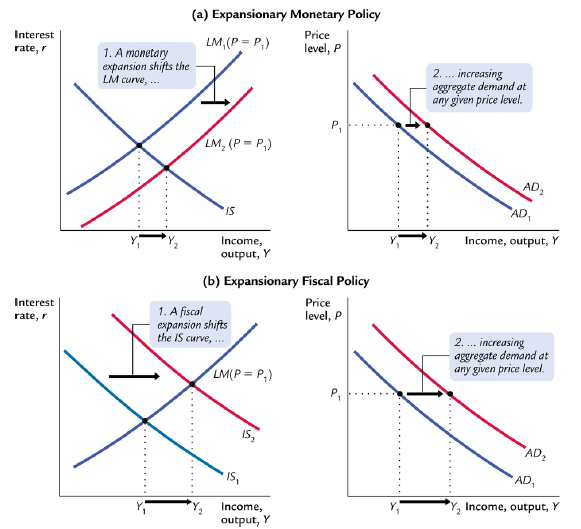
\includegraphics[width=\linewidth]{AD}
					\caption{从IS-LM到AD}
				\end{minipage}
			}\
			\hfill
			\subfloat[]{
				\begin{minipage}[b]{0.36\linewidth}
					\centering
					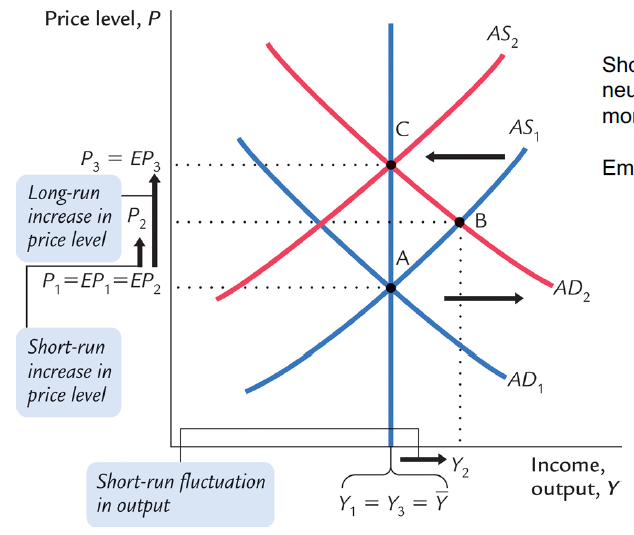
\includegraphics[width=\linewidth]{AS-AD}
					\caption{AS-AD}
				\end{minipage}
			}
		\end{minipage}
	\end{figure}
\end{center}
\subsection{Phillips Curve}
衡量失业率与通胀的模型. \textbf{Inflation} depends on expected inflation, cyclical unemployment, and supply shocks.
\paragraph{Okun’s law} 失业率的上升伴随着GDP的下降, 设自然失业率为$u^n$
$$Y - \overline{Y} = -\gamma (u - u^n)$$
失业率变动1\%使得GDP变动2\%.

从\textbf{总供给曲线(AS)}推导:
$$Y = \overline{Y} + \alpha(P-EP) = \overline{Y} + \alpha P_{-1}(\frac{P-P_{-1}}{P_{-1}} - \frac{EP-P_{-1}}{P_{-1}})$$
因为$\pi = \frac{P-P_{-1}}{P_{-1}}$, $E\pi =\frac{EP-P_{-1}}{P_{-1}} $
所以
$$Y - \overline{Y} = \alpha P_{-1}(\pi - E\pi)$$
引入供给冲击$v$, 负影响:
$$Y - \overline{Y} = \alpha P_{-1}(\pi - E\pi - v)$$
应用Okun’s law:
$$-\gamma (u - u^n) = \alpha P_{-1}(\pi - E\pi - v)$$
整理得到($\beta = \gamma/(\alpha P_{-1})$):
$$\pi = E\pi - \beta(u - u^n) + v$$
\textbf{适应性预期:} $$E\pi = \pi_{-1}$$
所以得到
$$\pi = \pi_{-1} - \beta(u - u^n) + v$$
第一项为自然失业(通货膨胀预期,反映长期失业率),第二项为周期性失业,第三项为供给冲击; 高通胀预期意味着更高的Phillips曲线. 

实际上美国经济并不遵从,  因为在短期,通胀并不和预期通胀一致,  这导致Phillips曲线频繁地上下移动.
\paragraph{牺牲率(Sacrifice ratios)}
使通胀率降低1\%所放弃一年失业率的百分比. 典型的估计值为$5\%$

$E\pi$的定义决定牺牲率的计算方式,与前2年有关就要迭代2次,因为$E\pi$要2年后才能稳定.
\begin{center}
	\begin{figure}[htb] %强制单栏排版
		\centering %居中
		\begin{minipage}[b]{0.95\linewidth}
			\subfloat[]{
				\begin{minipage}[b]{0.46\linewidth} 
					\centering
					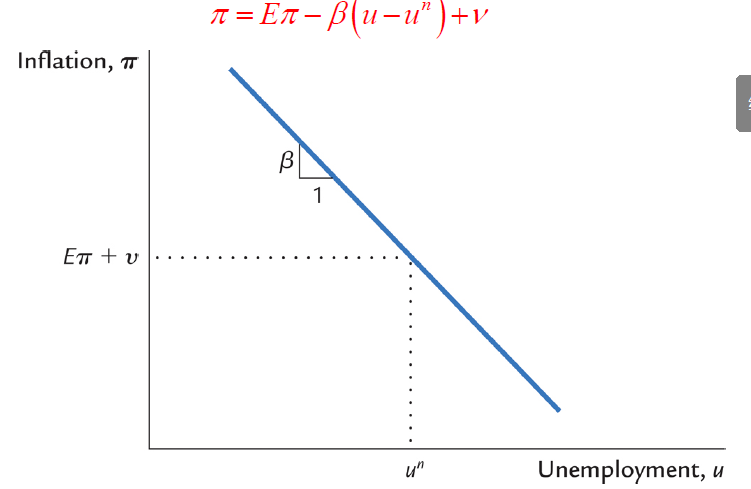
\includegraphics[width=\linewidth]{phili}
					\caption{Phillips curve}
				\end{minipage}
			}\
			\hfill
			\subfloat[]{
				\begin{minipage}[b]{0.45\linewidth}
					\centering
					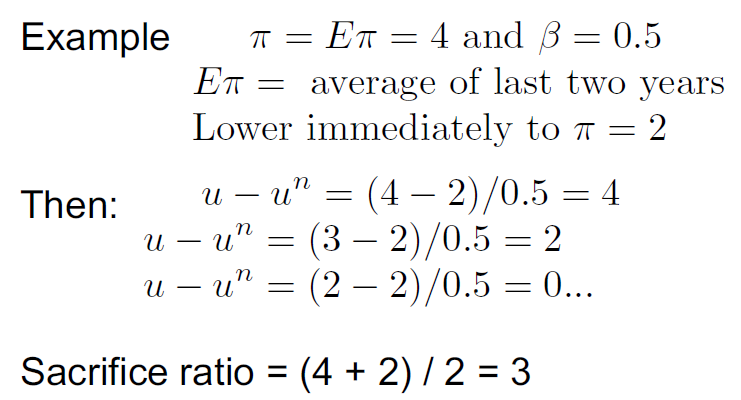
\includegraphics[width=\linewidth]{scari}
					\caption{Sacrifice ratios}
				\end{minipage}
			}
		\end{minipage}
	\end{figure}
\end{center}
\subsection{劳动力市场模型}
\textbf{变量:} W/P = MPL: 劳动力边际产量/劳动报酬;$H=L$: 劳动力总量; $C$:消费,代表福利; 税率:$\tau$

劳动力需求曲线: $W/P$上升,$L$需求减少.

劳动力供给曲线: $W/P$上升,$L$供给增加.

引入税收$T$: $T$增加,$L$供给减少.

使用Cobb-Douglas Production Function:
$$MPL = (1-\alpha)\frac{Y}{L} = \frac{W}{P}$$
家庭效用函数:
$$U(C, 100-H) = ln(C) + \theta ln(100-H)$$
均衡状态:
$$L = H$$
约束条件:
总消费 = 总收入:
$$C = (1-\tau)\frac{W}{P}H$$
得到最优化问题:
$$\max_{C, H}U(C, 100-H), PC = (1-\tau)WH$$
$$\max_{H} \ln((1-\tau)WH/P) + \theta\ln(100-H)$$
一阶条件:
$$\frac{(1-\tau)W/P}{C} - \frac{\theta}{100 - H} = 0$$
即
$$\frac{\theta C}{(1-\tau)(100 - H)} = \frac{W}{P} = MPL = (1-\alpha)\frac{Y}{H(=L)}$$
解得均衡劳动力总量:
$$H = 100\left(\frac{1-\alpha}{1 - \alpha + \frac{C}{Y}\frac{\theta}{1-\tau}}\right)$$

\textbf{引入消费税$\tau^C$}

约束条件:
$$(1+\tau^C)C = (1-\tau)\frac{W}{P}H$$
即$$(1+\tau^C)PC = (1-\tau)WH$$
带入上述模型即可.

\subsection{Unemployment}
\paragraph{工资刚性}
工资未能调整到劳动供给 =  劳动需求的水平。(工资并不总是由弹性的,有时停滞在高于市场出清的水平,使得供给>需求)
\paragraph{摩擦性失业(frictional)} 工人找工作需要花时间而引起的失业. $U^F$.
 原因之一:部门转移(sectoral shift). 需求在不同行业和地区之间变动.
 
\textbf{ 失业保障}增加了摩擦性失业,因为减轻了失业的经济困难.
\paragraph{结构性失业(structural)} 工资刚性和工作配给引起的失业. $U^S$

\textbf{最低工资法}可以造成工资刚性,加剧了结构性失业.

\textbf{税收抵免}可以防止穷人太穷,但是会减少政府税收收入.

\paragraph{周期性失业(Cyclical)}
短期现象,随经济周期波动.

设短期实际失业人数为$U$, 则满足下述公式:
$$U = U - U^N + U^F + U^S, U^N = U^F + U^S$$
令离职率(separation):$s$, 入职率(finding):$f$.
\begin{figure}[htb]
	\centering
	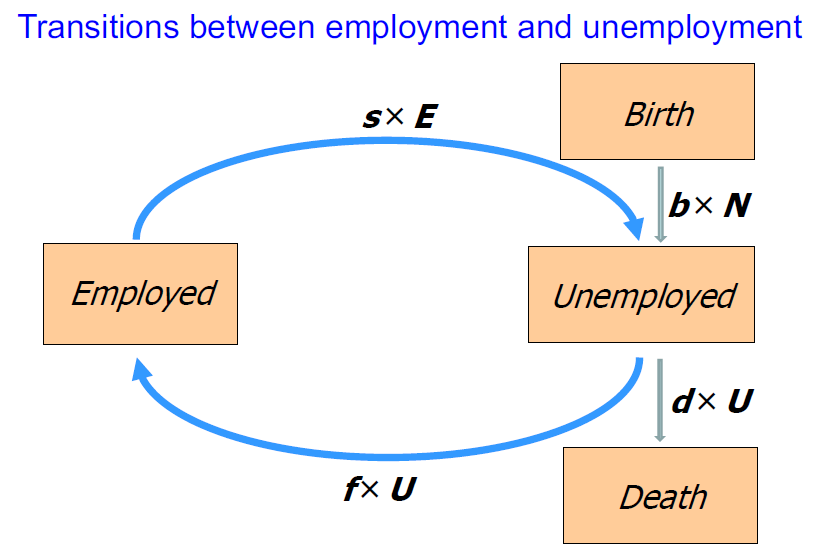
\includegraphics[width=0.5\linewidth]{employ}
\end{figure}
\paragraph{Model of Job Search}
U: 失业人数;I:劳动力市场人数(无工作/出生);X:退出市场人数(找到工作/死亡);N = L:劳动力总量.

b: 出生率;d: 死亡率;s: 离职率;f: 入职率; u: 失业率(=U/N); $1/f$: 期望失业时间.
$$\triangle U = I - X$$
$$I = bN + s(N-U)$$
$$X = dU + fU$$
$$\frac{\triangle N}{N} = b - d$$
推导动态变化:
$$\triangle u/u = \triangle U/U - \triangle N/N = \frac{I-X}{U} - (b-d) = \frac{bN + s(N-U) - dU - fU}{U} - b + d = (b+s)\frac{N}{U} -s -d-f-b+d$$
进而得到:
$$\triangle u = b+s - (b+s+f)u$$
\textbf{和死亡率无关!}

\textbf{稳态:}
$$u^* = \frac{b+s}{b+s+f} = 1 - \frac{f}{b+s+f}$$
\paragraph{关于$f$的决定论}
$f$取决于三者: 职位空缺(vacancies)$v$, 找工作强度(intensity of search)$i$, 工作匹配度(ease of matching)$m$. 即$f = f(v, i, m)$
三者均对$f$有正贡献.
$$u^* = \frac{b+s}{b+s + f(v, i, m)}$$
\paragraph{Beveridge Curve}v-u: 贝弗里奇曲线(BV).

$v$增加,$f$增加,$u$下降.
\paragraph{Job Creation Curve}(v-u) 职位供给曲线(JC).
两个事实:

$\bullet$ 更高的失业率降低工资: 因为降低了工会议价能力、劳动力需求曲线决定、效率工资降低(高失业率使得离职的成本变高,因此企业可以降低工资)

$\bullet$低工资升高职位空缺率$v$. 

所以高失业率$u$将提高职位空缺率$v$.

$\bullet$ 慷慨的失业保险: 降低$i$

$\bullet$ 就业保障: 降低$s$(BV曲线左移),降低$v$(JC曲线).
\begin{center}
	\begin{figure}[htb] %强制单栏排版
		\centering %居中
		\begin{minipage}[b]{0.95\linewidth}
			\subfloat[]{
				\begin{minipage}[b]{0.4\linewidth} 
					\centering
					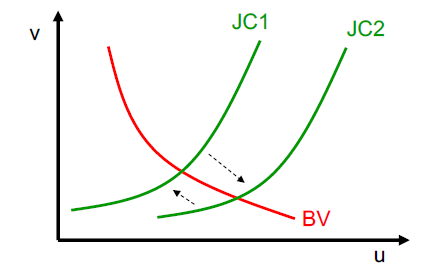
\includegraphics[width=\linewidth]{BV-JC}
					\caption{BV-JC curve}
				\end{minipage}
			}\
			\hfill
			\subfloat[]{
				\begin{minipage}[b]{0.52\linewidth}
					\centering
					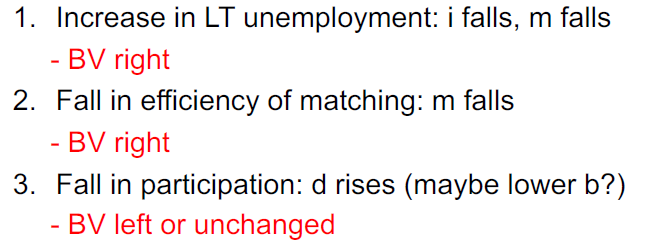
\includegraphics[width=\linewidth]{disc}
				\end{minipage}
			}
		\end{minipage}
	\end{figure}
\end{center}
\subsection{两期模型}
投资与消费的跨期选择问题.
Period 1:
$$c_1 + s = y_1$$
Period 2:
$$c_2 = y_2 + (1+r)s$$
得到\textbf{Budget constraint}
$$c_1 +\frac{c_2}{1+r} = y_1 + \frac{y_2}{1+r} = w$$
\begin{figure}[htb]
	\centering
	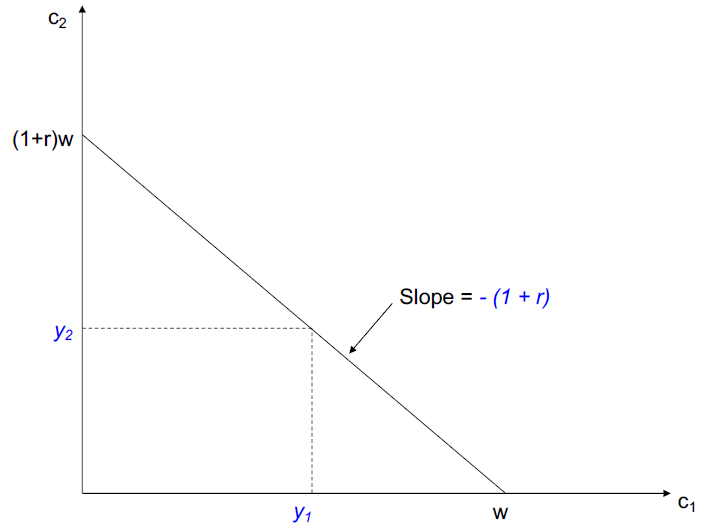
\includegraphics[width=0.35\linewidth]{budget}
\end{figure}
效用函数:
$$U = \ln c_1 + \beta \ln c_2$$
$\beta$越大说明耐心越大.

最优选择满足Euler equation(财富或收入不会影响消费的增长率):
$$\frac{c_2}{c_1} = \beta(1+r)$$
$$c_1 = \frac{w}{1+\beta}, c_2 = \frac{\beta(1+r)}{1+\beta}w$$
\textbf{引入税收$\tau$:}
$$c_1 + s = y_1 - \tau_1$$
$$c_2 = y_2 +(1+r)s - \tau_2$$
得到:
$$c_1 +\frac{c_2}{1+r} = w = y_1 - \tau_1 +\frac{y_2 - \tau_2}{1+r}$$
\textbf{lump-sum tax}没有税收扭曲效应,满足Euler equation.
得到最优解:
$$c_1 = \frac{w}{1+\beta},\quad c_2 = \frac{(1+r)\beta}{1+\beta}w$$
\textbf{引入消费税$\tau^c$:}
$$(1+\tau_1)c_1 +s = y_1$$
$$(1+\tau)c_2 = y_2 + (1+r)s$$
得到:
$$(1+\tau_1)c_1 + \frac{(1+\tau_2)c_2}{1+r} = y_1+\frac{y_2}{1+r} = w$$
一阶条件:
$$\frac{c_2}{c_1} = \beta(1+r)\frac{1+\tau_1}{1+\tau_2}$$
\textbf{distorting-tax} 有扭曲现象,只有相等才满足Euler equation.

\textbf{Tax smoothing:} Want to set $\tau_1 = \tau_2$ smooth taxes over time.

\textbf{政府两期模型:}
$$g_1 = \tau_1 + b$$
$$g_2 + (1+r)b = \tau_2$$
$b$是政府借款/发行债券的收入.

考虑\textbf{产品有耐用性},折旧率$\delta$:
$$U = ln(C_1) + \beta ln(C_2 + (1 - \delta)C_1)$$
$$c_1 + \frac{c_2}{1+r} = w = Y_1 + \frac{Y_2}{1+r}$$
得到最优解:
$$C_1 = \frac{r+1}{(\beta+1)(r+\delta)}w$$
$$C_2 = \frac{r+1}{(\beta+1)(r+\delta)}\left[\beta(r+\delta)+\delta-1\right]w$$
$\delta=1$时退化到普通情形.
$$\frac{\triangle C_1}{\triangle Y_1} = \frac{r+1}{(\beta+1)(r+\delta)}$$
$$\frac{\triangle C_2}{\triangle Y_2} = \frac{\beta(r+\delta)+\delta-1}{(\beta+1)(r+\delta)}$$
$$TB_1 = Y_1 - C_1 = \frac{\beta(r+\delta)+\delta-1}{(\beta+1)(r+\delta)}Y_1 - \frac{1}{(\beta+1)(r+\delta)}Y_2$$
$$TB_2 = Y_2 - C_2 = -(1+r)TB_1 = \frac{1+r}{(\beta+1)(r+\delta)}Y_2 - (1+r)\frac{\beta(r+\delta)+\delta-1}{(\beta+1)(r+\delta)}Y_1$$
$$\frac{\triangle TB_1}{\triangle Y_1} = \frac{\beta(r+\delta)+\delta-1}{(\beta+1)(r+\delta)}$$
$$\frac{\triangle TB_2}{\triangle Y_2} = \frac{1+r}{(\beta+1)(r+\delta)}$$
令上式$\triangle TB_1 / \triangle Y_1 = 0$得到临界逆周期(Countercyclicality)折旧率:
$$\delta_0 = \frac{1-\beta r}{1+\beta}$$
$\delta > \delta_0$时, 折旧偏多,极端情况是基础情形,$TB_1$顺周期.
$Y_1$增加时,使得HouseHold Wealth $w$增加,使得消费增加,而$C_1$只占$w$的一部分,所以$\triangle C_1 < \triangle Y_1$, 所以$TB_1$随着$Y_1$的增加而增加.
如果没有折旧,即$\delta = 0$, 那么一期商品将延续到二期, 那么人们可能存在超前消费,$C_1$的支出可能会超过$Y_1$, $\triangle(Y_1-C_1) < 0$, 此时$TB_1 < 0$, 是逆周期变动的.
\paragraph{Ricardian Equivalence Theorem(李嘉图等价定理)}
征税和政府借款在逻辑上是相同的。
$$\tau + \frac{\tau}{1+r} = g_1 + \frac{g_2}{1+r}$$
\subsection{开放经济体}
$$Y = C+G+I +X-M$$
Debt: $B_t$, 初始赤字(primary deficit): $D_t$。 Debt sustainability:
$$\triangle B_t = r_tB_t + D_t$$
Debt / nominal-GDP (g为GDP增长率,$\pi$为通胀率):
$$b = \frac{B_t}{PY_t}$$
$$\frac{\triangle b}{b} = \frac{\triangle B}{B} - \frac{\triangle P}{P} - \frac{\triangle Y}{Y} = r + \frac{D}{B} - \pi - g$$
即:
$$\triangle b/b = \frac{D}{B} - (\pi + g - r)$$
\textbf{TB: Trade Balance}
$$TB = ExportGoods - ImportsGoods$$
\textbf{CA: Current Account}
$$\sum_{country\in world}CA = 0$$
\textbf{NIIP:Net International Investment Position}
$$NIIP = A - L$$
$$\sum_{country\in world}NIIP = 0$$
$$\triangle NIIP = CA + ValuationChanges$$
$\triangle NIIP$是零和的.

\textbf{开放经济的两期模型:}

没有$G, I$时:
$$TB_1 = Y_1 - C_1 = B_1 - (1+r_0)B_0$$
$$CA_1 = B_1 - B_0$$
$$C_1+B_1 = (1+r_0)B_0 + Y_1$$
$$C_2+B_2 = (1+r_1)B_1 + Y_2$$
$$B_2 = 0$$
得到
$$C_1 +\frac{C_2}{1+r_1} = (1+r_0)B_0 + Y_1 + \frac{Y_2}{1+r_1} = w$$
没有Valuation Changes(估值变动)时:
$$CA_1 = \triangle NIIP = B_1 - B_0 = S_1 - I_1 = TB_1 + rB_0$$
$$Y = C + G + I + TB_1 = C+G+I + CA_1 - rB_0$$
$$GNP = C+G+I+CA_1$$
\textbf{Terms-of-Trade}
出口商品价格/进口商品价格
$$TT = \frac{P^X}{P^M}$$
两期模型:
$$P_1^MC_1 + P_1^MB_1 = P_1^M(1+r_0)B_0 + P_1^XY_1$$
进而 得到:
$$C_1+B_1 = (1+r_0)B_0 + TT_1Y_1$$
$$C_2+B_2 = (1+r_1)B_1 + TT_2Y_2$$
budget constraint:
$$C_1 +\frac{C_2}{1+r_1} = (1+r_0)B_0 + TT_1Y_1 + \frac{TT_2Y_2}{1+r_1} = w$$
\textbf{重要公式:}
$$TB_1 = Y_1 - C_1 = B_1 - (1+r_0)B_0$$
$$CA_1 = B_1 - B_0$$
美国NIIP和NII(Net investment income)之间的巨大差别:
\textbf{Dark Matter and Return Differentials}
回报率的差别:
$$NII = r^AA - r^LL$$
Dark Matter:
$$NII = r*TNIIP, DarkMatter = TNIIP - NIIP$$
\end{document}